\section{Trig}
	\subsection{Trigonometric Formulas}
	\begin{multicols}{2}
	\noindent
	\begin{equation}
	\label{sin}
	sin^2x=\frac{1-\cos{2x}}{2}
	\end{equation}
	\begin{equation}
	cos^2x=\frac{1+\cos{2x}}{2}
	\end{equation}
	\end{multicols}
	
	\begin{simple}{}{}
	Find
	$$\int\sin^2{(x)}dx$$
	using trigonometric formulas \ref{sin}:
	\begin{align*}
	    \int\sin^2{(x)}dx&=\int\frac{1-\cos{(2x)}}{2}dx\\
	    &=\frac{1}{2}\int(1-\cos{(2x)})dx\\
	    &=\frac{1}{2}\left[\int1dx-\int\cos{(2x)}dx\right]\\
	    &=\frac{1}{2}\left[x-\int\cos{(2x)}dx\right]\\
	\end{align*}
	
	Let $u=2x$, so that $\frac{du}{dx}=2$
	\begin{align*}
	    \int\cos{(2x)}dx&=\frac{1}{2}\int\cos{(u)}du\\
	    &=\frac{1}{2}\sin{(u)}\\
	    &=\frac{1}{2}\sin{(2x)}+C
	\end{align*}
	
	Back the the equation above:
	\begin{align*}
	    &=\frac{1}{2}\left[x-\int\cos{(2x)}dx\right]\\
	    &=\frac{1}{2}\left[x-\frac{1}{2}\sin{(2x)}\right]+C\\
	    &=\frac{1}{2}x-\frac{1}{4}\sin{(2x)}+C
	\end{align*}
	\end{simple}
	
	\subsection{Application In Integration}
	\begin{equation}
	\int\sin^2{x}\ dx=\frac{1}{2}x-\frac{1}{4}\sin{2x}+C
	\end{equation}
	\begin{equation}
	\int\cos^2{x}\ dx=\frac{1}{2}x+\frac{1}{4}\sin{2x}+C
	\end{equation}
	
	It is strongly recommended that you remember these two equations.
	
	\subsection{Inverse Trigonometry}
	
	\begin{equation}
	\int\frac{1}{\sqrt{a^2-u^2}}\ du=\sin^{-1}\left(\frac{u}{a}\right)+C
	\end{equation}
	\begin{equation}
	\int\frac{1}{a^2+u^2}\ du=\frac{1}{a}\tan^{-1}\left(\frac{u}{a}\right)+C
	\end{equation}
	\begin{equation}
	\int\frac{1}{u\sqrt{u^2-a^2}}\ du=\frac{1}{a}\sec^{-1}\left(\frac{u}{a}\right)+C
	\end{equation}
	
	\subsection{Reduction Formula}
	\begin{equation}
	\int\sin^n{x}\ dx=\frac{1}{n}\cos{x}\sin^{n-1}{x}+\frac{n-1}{n}\int\sin^{n-2}{x}\ dx
	\end{equation}
	\begin{equation}
	\int\cos^nx\ dx=\frac{1}{n}\sin{x}\cos^{n-1}x+\frac{n-1}{n}\int\cos^{n-2}x\ dx
	\end{equation}
	
	\begin{simple}{}{}
	Find 
	$$\int \sin^4{(x)} dx$$
	using reduction formula
	
	Solution:
	\begin{align*}
	    \int \sin^4{(x)}&=\frac{1}{4}\cos{(x)}\sin^{4-1}{(x)}+\frac{4-1}{4}\int \sin^{4-2}{(x)}dx\\
	    &=\frac{1}{4}\cos{(x)}\sin^3{(x)}+\frac{3}{4}\int \sin^2{(x)}dx\\
	    &=\frac{1}{4}\cos{(x)}\sin^3{(x)}+\frac{3}{4}*\left(\frac{1}{2}x-\frac{1}{4}\sin{(2x)}\right)+C\\
	    &=\frac{1}{4}\cos{(x)}\sin^3{(x)}+\frac{3}{8}x-\frac{3}{16}\sin{(2x)}+C
	\end{align*}
	\end{simple}
	
	\subsection{Double Angle Formula}
	\begin{equation}
	2\sin\theta\cos\theta\ =\ \sin{2\theta}
	\end{equation}
	
	\subsection{Products Of Sin and Cos}
	\begin{center}
	Let A and B represent real number
	\end{center}
	\begin{equation}
	\sin{(Ax)}\cos{(Bx)}=\frac{1}{2} \left( \sin{(Ax-Bx)}+\sin{(Ax+B)}\right)
	\end{equation}
	\begin{equation}
	\sin{(Ax)}\sin{(Bx)}=\frac{1}{2}(\cos{(Ax-Bx)}-\cos{(Ax+Bx)})
	\end{equation}
	\begin{equation}
	\cos{(Ax)}\cos{(Bx)}=\frac{1}{2}(\cos{(Ax-Bx)}+cos{(Ax+Bx)})
	\end{equation}
	
	\subsection{Sub Into Trig}
	\begin{center}
	    \begin{equation}
	    \label{sin_trig}
    	\sqrt{c^2-x^2}\text{\ \ \ \ } Let\ x=c\sin{(\theta )}\text{\ \ \ \ } \sqrt{c^2-x^2}=c\cos{(\theta )}
    	\end{equation}
    	\begin{figure}[H]
    	\center
    	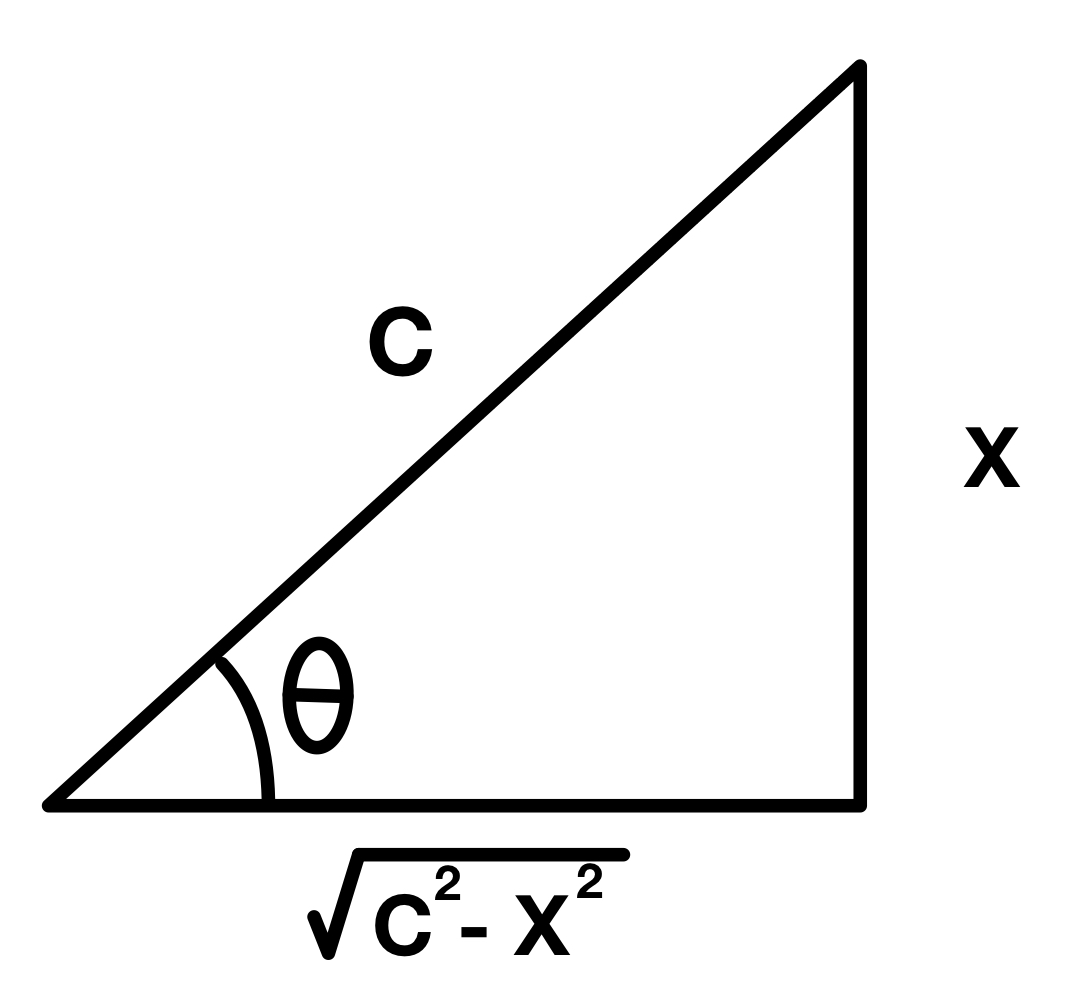
\includegraphics[width=4cm]{Pictures/sin}
    	\end{figure}
    	
    	\begin{equation}
    	\sqrt{c^2+x^2}\text{\ \ \ \ } Let\ x=c\tan{(\theta )}\text{\ \ \ \ } \sqrt{c^2+x^2}=c\sec{(\theta )}
    	\end{equation}
    	\begin{figure}[H]
    	\center
    	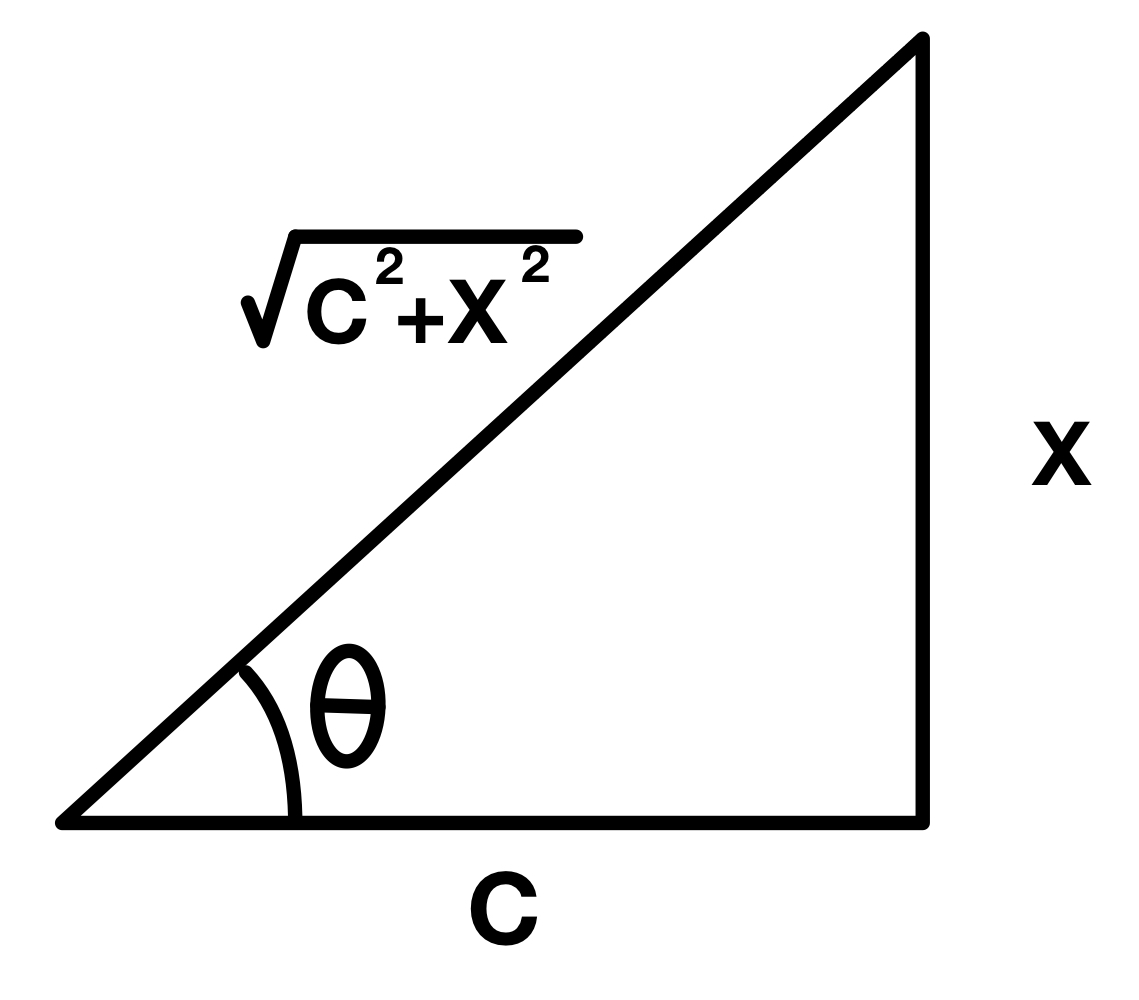
\includegraphics[width=4cm]{Pictures/tan.jpeg}
    	\end{figure}
    	
    	\begin{equation}
    	\sqrt{x^2-c^2}\text{\ \ \ \ } Let\ x=c\sec{(\theta )}\text{\ \ \ \ } \sqrt{x^2-c^2}=c\tan{(\theta )}
    	\end{equation}
    	\begin{figure}[H]
    	\center
    	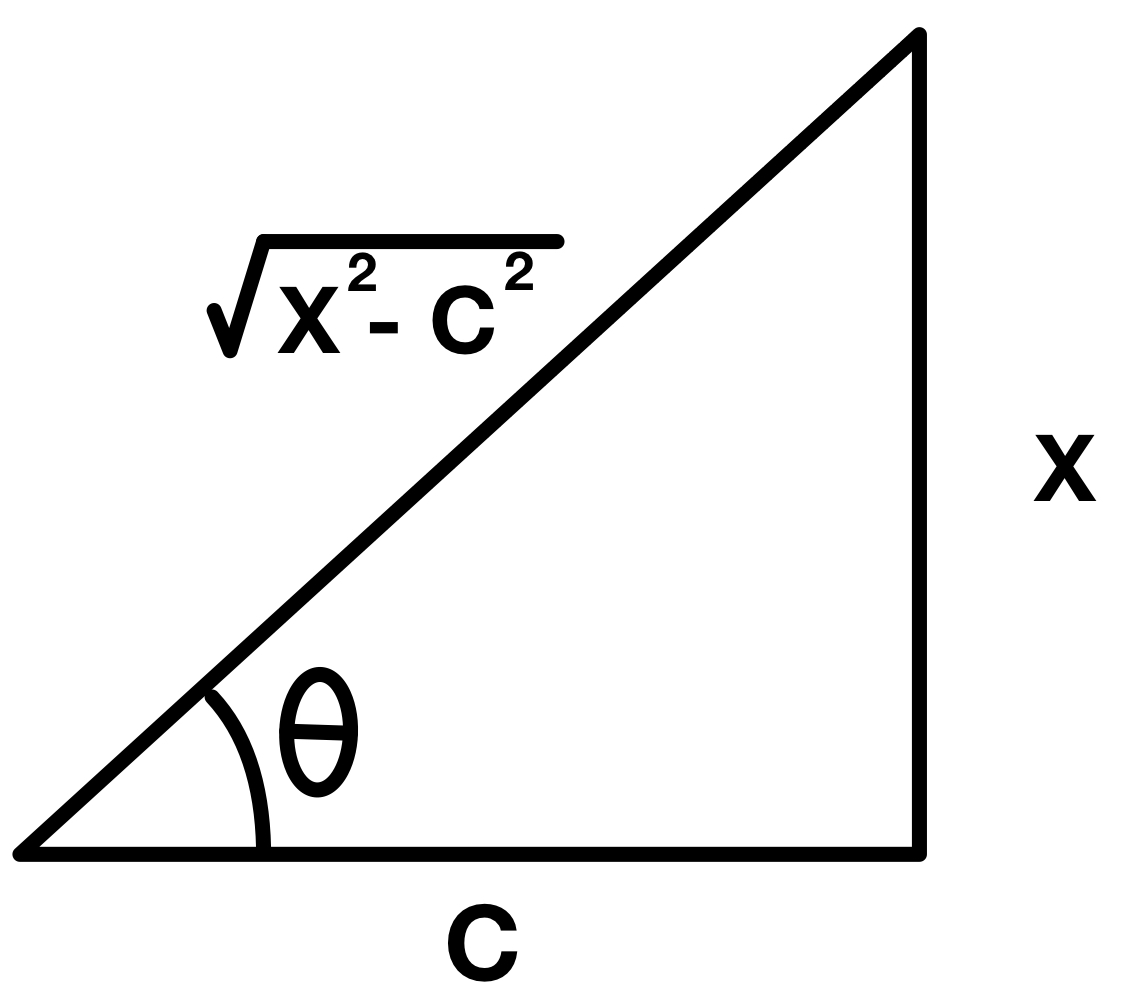
\includegraphics[width=4cm]{Pictures/sec}
    	\end{figure}
    	
    	\begin{simple}{}{}
    	Find
    	$$\int\sqrt{25-x^2}$$
    	
    	Let c=5, so that 
    	$$\int\sqrt{25-x^2}=\int\sqrt{5^2-x^2}$$
    	
    	Let $x=5\sin{(\theta)}$ and $\sqrt{5^2-x^2}=5\cos{(\theta)}$
    	so that $\dfrac{dx}{d\theta}=5\cos{(\theta)}$
    	and $\theta=\sin^-1{(\frac{x}{5})}$
    	
    	\begin{align*}
    	    \int\sqrt{5^2-x^2}dx&=\int5\cos{(\theta)}*5\cos{(\theta)}d\theta\\
    	    &=25\int\cos^2{(\theta)}\\
    	    &=25*\left(\frac{1}{2}\theta+\frac{1}{4}\sin{(2\theta)}\right)\\
    	    &=25*\left(\frac{1}{2}\theta+\frac{1}{4}*2*\sin{(\theta)}*\cos{(\theta)}\right)\\
    	\end{align*}
    	Look at the triangle from theorem \ref{sin_trig}, we can see that $\sin{(\theta)}=\frac{x}{c}$ and $\cos{(\theta)}=\frac{\sqrt{5^2-x^2}}{5}$
    	
    	\begin{align*}
    	    25\left(\frac{1}{2}\theta+\frac{1}{4}*2*\sin{(x)}*\cos{(\theta)}\right)&=25\left(\frac{1}{2}\sin^{-1}{(x)}+\frac{1}{2}*\left(\frac{x}{5}\right)*\left(\frac{\sqrt{5^2-x^2}}{5}\right)\right)\\
    	    &=25\left(\frac{1}{2}\sin^{-1}{(\frac{x}{5})}+\frac{1}{50}x\sqrt{25-x^2}\right)
    	\end{align*}
    	
    	\end{simple}
    	
    	\begin{example}{}{}
    	Find
    	$$\int x\sqrt{16-2x^2}dx$$
    	
    	Let $c=4$ and $u=\sqrt{2}x$, so that $\dfrac{du}{dx}=\sqrt{2}$
    	
    	$$\int x\sqrt{16-2x^2}dx=\frac{1}{2}\int u\sqrt{4^2-u^2}du\\$$
    	
    	Let $u=4\sin{(\theta)}$ and $\sqrt{4^2-u^2}=4\cos{(\theta)}$
    	
    	so that $\dfrac{du}{d\theta}=4\cos{(\theta)}$
    	
    	\begin{align*}
    	    \frac{1}{2}\int u\sqrt{4^2-u^2}du&=\frac{1}{2}\int 4\sin{(\theta)}*4\cos{(\theta)}*4\cos{(\theta)}d\theta\\
    	    &=32\int\sin{(\theta)}\cos^2{(\theta)}d\theta\\
    	\end{align*}
    	Let $v=\cos{(\theta)}$, so that $\frac{dv}{d\theta}=-\sin{(\theta)}$
    	\begin{align*}
    	    32\int\sin{(\theta)}\cos^2{(\theta)}d\theta&=-32\int v^2 dv\\
    	    &=-32*\frac{1}{3}v^3+C\\
    	    &=-\frac{32}{3}v^3+C\\
    	    &=-\frac{32}{3}\cos^3{(\theta)}+C\\
    	\end{align*}
    	
    	Looking at the image of equation \ref{sin_trig}, we observe that
    	$$\cos{(\theta)}=\frac{\sqrt{c^2-x^2}}{c}$$
    	
    	%\begin{figure}[H]
    	%    \centering
    	%    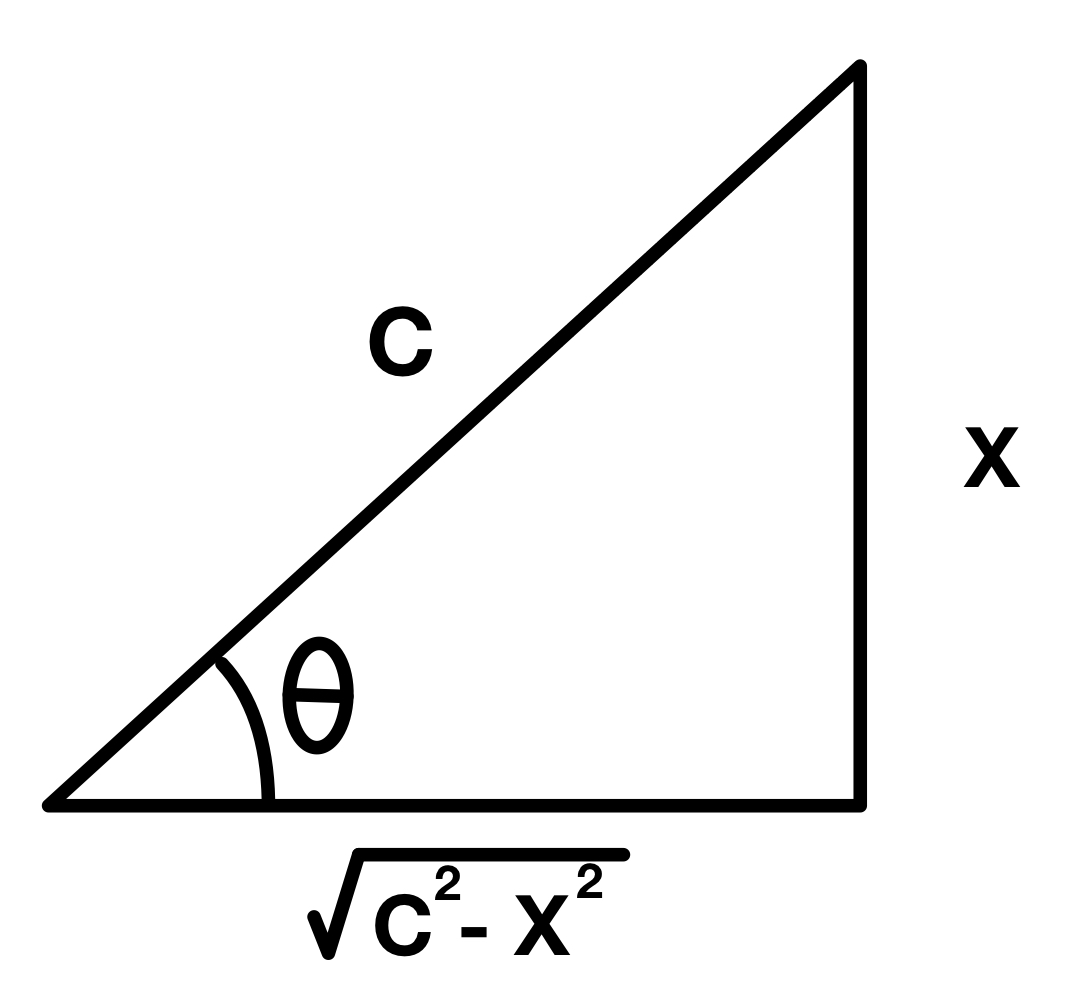
\includegraphics[width=3cm]{Pictures/sin.jpeg}
    	%\end{figure}
    	
    	\begin{align*}
    	    -\frac{32}{3}\cos^3{(\theta)}&=-\frac{32}{3}*\left(\frac{\sqrt{4^2-u^2}}{4}\right)^3\\
    	    &=-\frac{32}{3}*\left(\frac{\sqrt{16-2x^2}}{4}\right)^3\\
    	    &=-\frac{1}{6}*\left(\sqrt{16-2x^2}\right)^3
    	\end{align*}
    	or use u-substitution lol.
    	\end{example}
    	
    	\begin{example}{}{}
    	Find
    	$$\int \frac{x^2}{\left(4-x^2\right)^\frac{3}{2}}dx$$
    	
    	Let $x=2\sin{(\theta)}$ and $\sqrt{4-x^2}=2\cos{(\theta)}$
    	
    	so that $\theta=\sin^{-1}{(x)}$, $\dfrac{dx}{d\theta}=2\cos{(\theta)}$
    	
    	\begin{align*}
    	    \int \frac{x^2}{\left(4-x^2\right)^\frac{3}{2}}dx&=\int \frac{4\sin^2{(\theta)}}{8\cos^3{(\theta)}}*2\cos{(\theta)}d\theta\\
    	    &=\int\frac{8\sin^2{(\theta)\cos{(\theta)}}}{8\cos^3{(\theta)}}d\theta\\
    	    &=\int\frac{\sin^2{(\theta)}}{\cos^2{(\theta)}}d\theta\\
    	    &=\int \tan^2{(\theta)}d\theta\\
    	    &=\int \left(\sec^2{(\theta)}-1\right)d\theta\\
    	    &=\tan{(\theta)}-\theta+C
    	\end{align*}
    	
    	Take a look back into the triangle in equation \ref{sin_trig}, we notice that $\tan{(\theta)}=\dfrac{x}{\sqrt{4-x^2}}$
    	
    	$$\tan{(\theta)}-\theta+C=\tan{(\theta)}=\dfrac{x}{\sqrt{4-x^2}}-\sin^{-1}{\left(\frac{x}{2}\right)}+C$$
    	\end{example}
	\end{center}
	